\section{Adjacent Ideas and Ecological Adoptions}

[I want to use this section of the paper to discuss some of the other disciplines that have taken up ecological ideas or themes. My hope is that this discussion may help show how information science can benefit from ecological thinking, and to possibly suggest improvements in the application of ecological ideas to the field of information science.] [take this paragraph out?]

Ecological concepts have been adopted by many different disciplines over the course of the twentieth century (see figure 2). An examination of some of these adoptions may help to illuminate the adoption of those ideas into information studies in the late 1990s. Three examples of ecological concepts migrating into other disciplines will be discussed in this section: cognitive ecology, media ecology, and political ecology. Each of them shows how ecological concepts can be adopted by a discipline for many different purposes. Purposes which may be renegotiated at any time.

\begin{figure}[!ht]
  \centering
    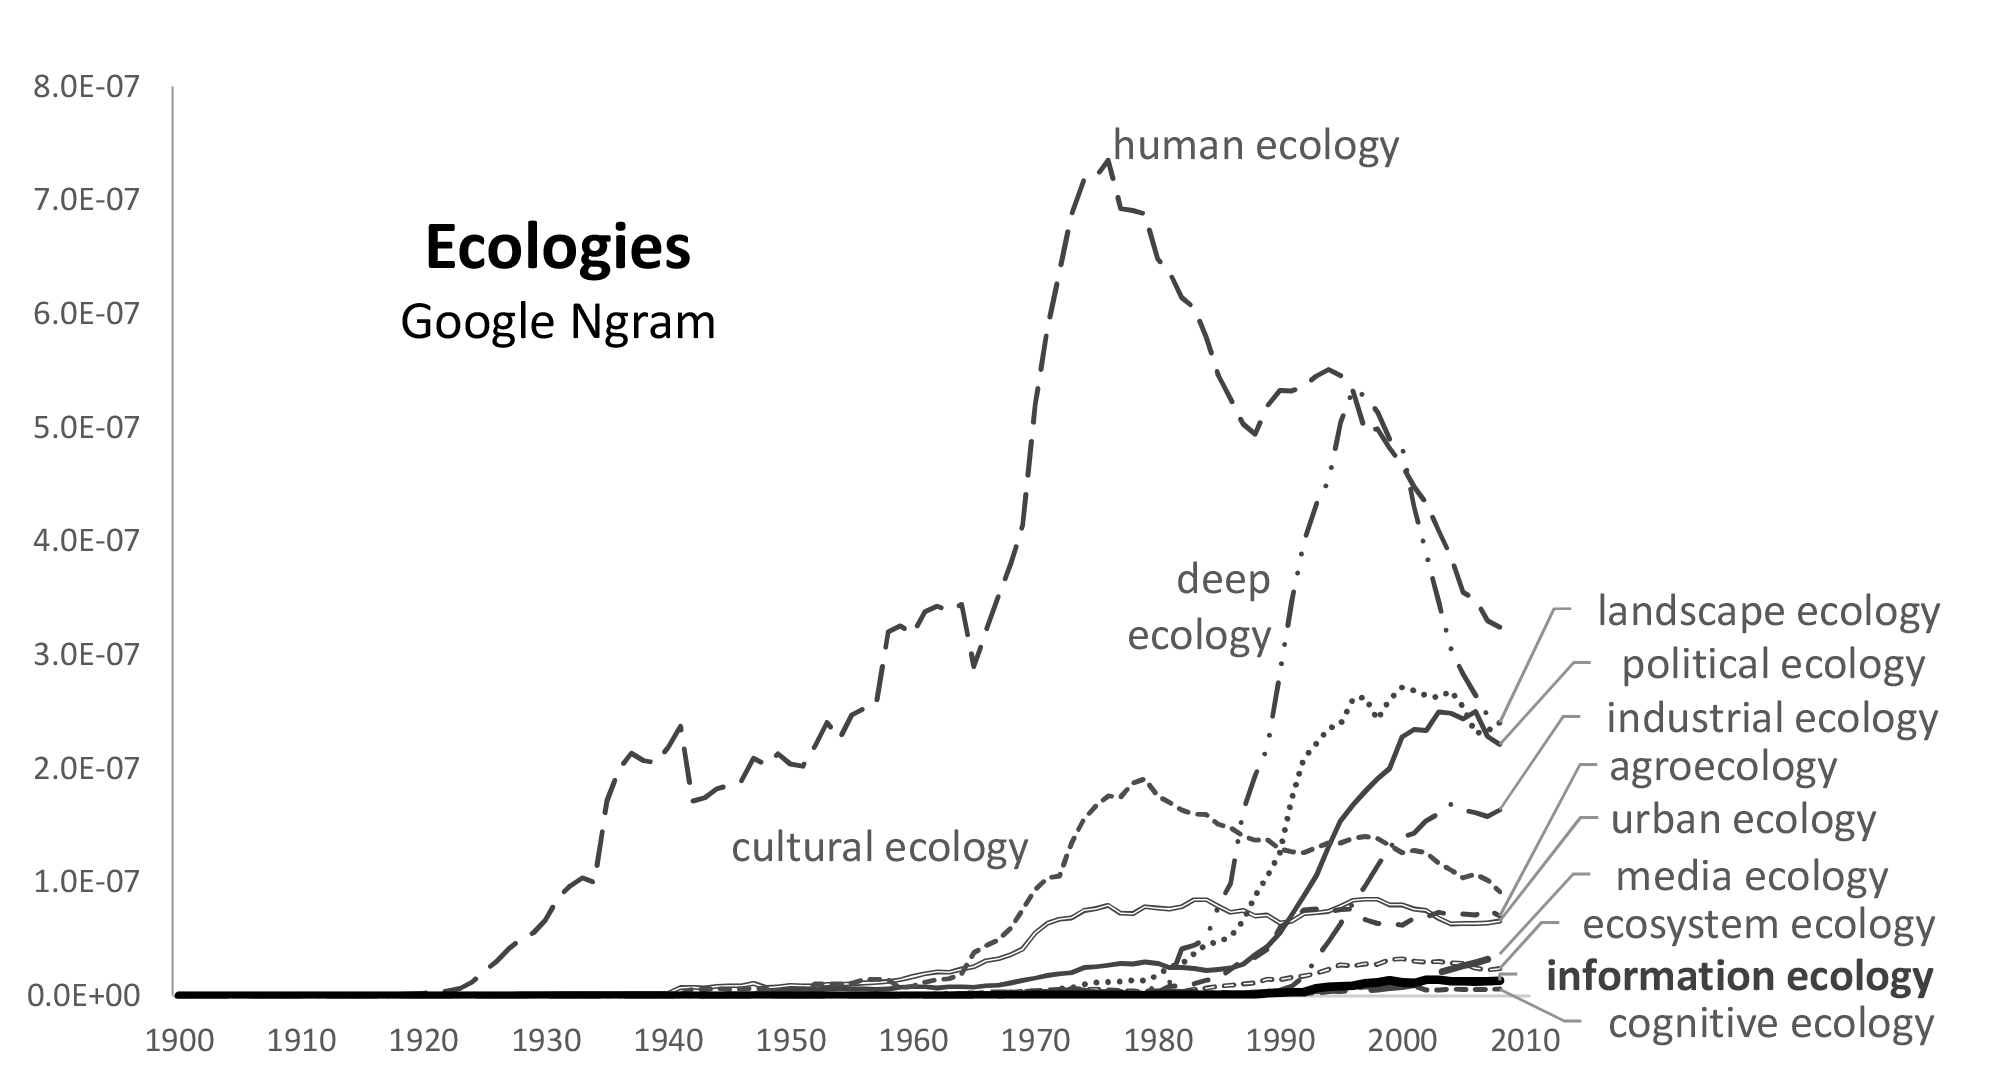
\includegraphics[width=5.5in]{figures/ecologiesAll}
  \caption{Emergent ecologies as a Google Ngram. Note the early dominance of human ecology and then deep ecology; only in the 1990s did ecological thinking become broadly adopted in many disciplines.}
\end{figure}

\subsection{Cognitive Ecology}

In a review of cognitive ecology Hutchins \citep{hutchins_cognitive_2010} discusses the sources of the field and how it interacts with cognitive science. He writes that "Cognitive ecology is the study of cognitive phenomena in context. Elements of cognitive ecology have been present in various corners, but not the core, of cognitive science since the birth of the field. It is now being rediscovered as cognitive science shifts from viewing cognition as a logical process to seeing it as a biological phenomenon." (705) In the abstract he highlights how cognitive ecology "points to the web of mutual dependence among elements of a cognitive ecosystem." [everything is connected? interconnectedness?]

A number of interesting rhetorical and thematic connections are being made in these statements. Hutchins contrasts logical and biological approaches to understanding cognition. Later in the paper he describes how early cognitive science was faced with a tension between reductionism and holism. Two schools of thought, a cybernetic and an information processing approach, emerged from the early ferment of the field. Cyberneticists, such as Gregory Bateson, emphasized the interactions between mind and the environment. Information processing advocates concentrated on the parallels between the digital computer and the mind. [make a diagram of this and use along with diagram of ecological economics? see below] The focus on the digital computer reduced the activity of the mind to symbolic event processing, relegating perceptual systems and the motor systems used to interact with the world to the periphery of the field of cognitive science. According to Hutchins, cognitive science is revising itself and reexamining the connections between the world and the mind. Cognitive ecology is an example of how these issues are being addressed.

Bateson wrote an influential book in 1972 titled \textit{Steps to an Ecology of Mind} \citep{bateson_1972}. The book was a theoretical manifesto for paying greater attention to the interconnections between environment and the mind. Other research programs emerged during the 1970s to form the base for cognitive ecology. Ecological psychology stressed the coupling between organism and environment, while cultural-historical activity theory stressed the internalization of inter-psychological processes during childhood development. Recent developments linking mind and environment have coalesced under the umbrella terms of embodied cognition and enaction. [Did he also write on "user resistance" to adoption of information systems??? see \citep{star_1996}]

One of the themes emerging from the development of cognitive ecology is the contrast between the digital and the biological. Cognitive science, as a field, chose to use a digital-technological paradigm in order to manage the scope of its studies and to define the appropriate units of analysis for its research efforts. Critics of this approach were present from the beginning, but often marginalized. A similar story is told by DP and NO in their narratives of information ecology, both of which employ the theme of moving away from a narrow technical focus on the systems for information management, which stand in for technological development, especially in the form of engineering with all of the symbolic baggage that term implies, toward a larger, contextually-dependent, vision of what information entails. Just as the cognitive ecologists wish to move away from viewing cognition as just another form of information processing, the information ecologists want to view the organization as something greater than a digital computer. Context becomes one of the key concepts for both motivating and operationalizing this transformation. Motivating because who would object to incorporating the context into a proper discussion of an information environment, and operationalizing because the idea of context points to a new unit of analysis beyond the individual software deployment toward the people and groups which surround and interact with any socio-technical system.

Another theme within Hutchins description of cognitive ecology is the idea of mutual dependence. NO use mutual dependence as one of their key themes within information ecology, and the interconnected organizations which surround a business are suggestive of the arguments made by DP. In \textit{Cognition in the Wild} Hutchins described the process used to navigate large Navy ships, which are excellent examples of the mutual dependence between people, technology, and information. Each component of the system, or [sic] ecology, needs to be functioning well in order to achieve the overall goal of determining the ship's position. Mutual dependence is also a principal feature within discourses about the value of biodiversity.

\subsection{Media Ecology}

Just as cognitive ecologists can trace back to original controversies over holism and reductionism, media ecologists can trace a similar debate in their own field of communication between qualitative and quantitative methods. Much of the early research in the field of communications tried to emulate the natural sciences and adopted quantitative methods from postwar social sciences. Early studies on propaganda and other communication topics adopted a simplistic view of information transmission, which was later derided as the hypodermic [what does this mean here?] or administrative model of communication. The scientistic view of communication would not be challenged until the 1960s and 1970s. Throughout this time there were researchers who approached media and communication studies from a critical point of view, including thinkers such as Marshall McLuhan, Walter Ong, and Neil Postman.

The network formed by McLuhan, Ong, and Postman is often cited as the foundation for media ecology studies. All three of these thinkers discussed the meaning of their own work and explicitly framed much of that work in environmental terms. Postman is usually credited with the earliest use of the term media ecology in a 1968 talk, later published in 1970. He defined media ecology as "the study of media as environments." \citep{strate_media_2004} McLuhan described the relationship between different types of media and how they effected the mental environment.

\begin{quote}
The medium is the message” means, in terms of the electronic age, that a totally new environment has been created. The “content” of this new environment is the old mechanized environment of the industrial age. The new environment
reprocesses the old one as radically as TV  is reprocessing the film. For the “content” of TV is the movie. TV is environmental and imperceptible, like all environments. We are aware only of the “content” or the old environment. When machine production was new, it gradually created an environment whose content was the old environment of agrarian life and the arts and crafts. This older environment was elevated to an art form by the new mechanical environment. The machine turned Nature into an art form [lets talk about this a little, perhaps it is a VERY important idea].\citep{mcluhan_understanding_2013} (p. 13)
\end{quote}

Ong writes about the "ecological concern" he believed media ecology would address, especially because "Its thrust is the dialectical opposite of the isolating thrust of writing and print." (p. 324) He described how evolutionary thinking proposed by Darwin demonstrated the development of organisms over time through the interaction of individuals and the environment. "The new philosophical attention to openness appears not unrelated to the opening of previously isolated human groups to one another fostered by electronic communications media, telephone, radio,
and ultimately television."\citep{ong_interfaces_1977} (p. 324)

Turning toward the environment in which communication and media interacted suggested a way to broaden the analysis of media in order to develop a broader critique of media in society. A more contemporary definition of media ecology is

\begin{quote}
how the form and inherent biases of communication media help create the environment or symbolic and cognitive structure in which people symbolically construct the world they come to know and understand, as well as its social, economic, political, and cultural consequences [but NOT environmental??]. \citep{lum_introduction:_2000}
\end{quote}

After the 1970s the study of media ecology spread in multiple directions. Ong focused on the distinction between orality and literacy, Postman became an influential public intellectual and critic of television, and McLuhan became famous his quote that the "medium is the message." Intellectual groups coalesced around many of these figures, especially in Toronto and New York, where McLuhan and Postman spent much of their careers [respectively?]. In 1998 the Media Ecology Association was established and solidified the use of the term media ecology. 

Two themes from media ecology are worth considering when examining the adoption of ecology into different disciplines. The first is the idea of the environment. McLuhan describes how technology has created a totally new environment in which people are now embedded. Moreover, the environment is often ignored or even imperceptible to the people who live in it [let's discuss this more]. There is a historical evolution of communication technologies in which older environments are replaced by newer ones. The second theme is raised by Ong when he talks about the openness engendered by the work of Darwin. Before Darwin species were considered separately from their environment, after the connections between individual and environment are paramount. Technology, in the form of electronic communication devices and networks, transforms human society in an analogous way, brining together groups which were previously isolated [but not people with the environment??].

\subsection{Political Ecology}

Political ecology is a fractious sub-discipline in the field of Geography that emerged in the later decades of the 20th century. Credit for the first use of the term is generally given to Eric Wolf in his 1972 article discussing environmental management in the Swiss Alps and how ownership of and access to resources structure environmental outcomes \citep{wolf_1972}. Very generally "[t]he phrase 'political ecology' combines the concerns of ecology and a broadly defined political economy. Together this encompasses the constantly shifting dialectic between society and the land-based resources, and also within classes and groups within society itself." \citep[][p. 17]{blaikie_1987}. Geography has close and enduring relationships with both ecology and political economy, but they tend to co-exist in non-harmonious ways. The emergence of political ecology represents an interdisciplinary effort to bring these two disciplines together; the "new"ecology as a reductionist approach to understanding nature and the Marxist critiques of political economy as a more holistic way of seeing human economic systems. This effort is but one of several projects within geography targeted to re-think human-nature relationships and outline programs for sustainability studies; aligned efforts include the social-ecological systems literature \citep{holling_2002} and the land-use land-change literature \citep{turner_2008}.

Often political ecology is defined not as a discipline but as an approach to understanding the degradation of socio-natural systems that puts historical, political and economic context at the forefront of any explanation. This approach became popular amongst scholars working in developing countries as an alternative to the standard development trope that population pressure begets degradation of natural resources and ecosystems. Alternatively, poverty and degradation are in a dialectical relationship that can spiral downwards if only one side is treated in policy \citep{blaikie_1987, peet_1996}. Political ecology also emerged as a critique of the small scale studies from human ecology and cultural ecology (see above), yet it retained the emphasis on the governance of, and access to, natural resources in the overall explanations of system dynamics. Indeed, often social justice is framed as an issue of access to and control of natural resources  through framings of property rights and regimes that range from constitutional to local, which then can be an explanatory factor for socio-natural outcomes. This property and access based approach also leads to alternative explanations of the tragedy of the commons thesis. Instead of inevitable degradation of the common "pasture" in Hardin's example--notably drawn from his work with bacteria in a petri dish, not people in a society--resources owned under common property regimes and governed by local practice and custom are often sustainably managed. While reminiscent of earlier human ecology, these alternate political ecological explanations fully acknowledge the problems of scale, complexity and context \citep{ostrom_1999}. 

A secondary, yet similarly powerful, framing of political ecology is that of the politics of environmental science. Also from thinkers involved in work in less developed countries, this framing explicitly gives science, and the knowledge, information and raw data that science produces, political agency in the policy arena. Instead of focusing on property regimes for managing natural resources, social justice is framed as an issue of the control of, access to and use of the scientific information \citep{forsyth_2003,leach_1996}. The work of Gregory Bateson in cognitive ecology was important in the development of political ecology conceived in this manner \citep{peet_1996}.

Together both of these framings draw heavily upon the narratives of ecologist as manager and the ecologist as activist. This has been heavily criticized, nevertheless. On the one hand, the approach is accused of being apolitical and only maintaining a superficial engagement with the political science literature \citep{walker_2007}. On the other hand, political ecology receives criticism for not including enough ecological thought and leaving explanations of environmental degradation to only political and economic factors \citep{vayda_1999,walker_2005}. In a sense political ecology fits well with Holling's observation that holistic approaches tend to offer answers of limited use to real problems \citep{holling_1998}. At the same time these two approaches provide traction for information ecology and how to embrace interdisciplinary attempts to solve "wicked problems" at planetary scales. It is perhaps this interdisciplinary engagement that all "ecologies" share that resonates most with and information ecology.

Political ecological approaches also provide alternative explanations to popular "success" stories of conquest and colonialism. Due to the explanatory power of guns, disease, and metallurgical technology as primary factors in the pro-colonial outcomes of the conquistadores in the New World \citep[cf.][]{diamond_1997}, attention to secondary factors is often overlooked. Political ecologists draw attention to non-primary factors of explanation such as the conquistadors desire for power, wealth and recognition. Without these secondary factors, the primary factors lose all explanatory power and the so-called superiority of European technology becomes only an enabler of actions that have little moral or ethical superiority. The "success" of the conquest was not a "natural" or "god-given" outcome as depicted through the idealism of manifest destiny in the United States, but instead a bloody tale of savagery and pillage. Additionally, common narratives of the colonial era often blame poverty and poor local land-management as primary drivers of environmental degradation. Alternatively, attention to material and economic flows towards the core (colonizing country) from the periphery (colonized country), advantageous labor costs in the colonies that drive the creation of poverty in indigenous populations, and devastating losses of embedded cultural knowledge about local ecosystem management, better explain the onset of environmental degradation.

\subsection{Ecologies vs Ecosystems}

Generally ecosystem metaphors--the information ecosystem, the urban ecosystem, the industrial ecosystem, and so on--are less used than the referents to the various ecologies--information ecology, cognitive ecology, political ecology and so on (see figure 3). Some confusion in the business management literature is introduced with the non-differentiation between the information ecosystem and information ecology. [is it true that "economy" can take both meanings; economy as the system and set of relations and economy as a discipline?? Perhaps "economics" as both a discipline and a set of relations? Is there a similarity with ecology here? Ecologics?]

\begin{figure}[!ht]
  \centering
    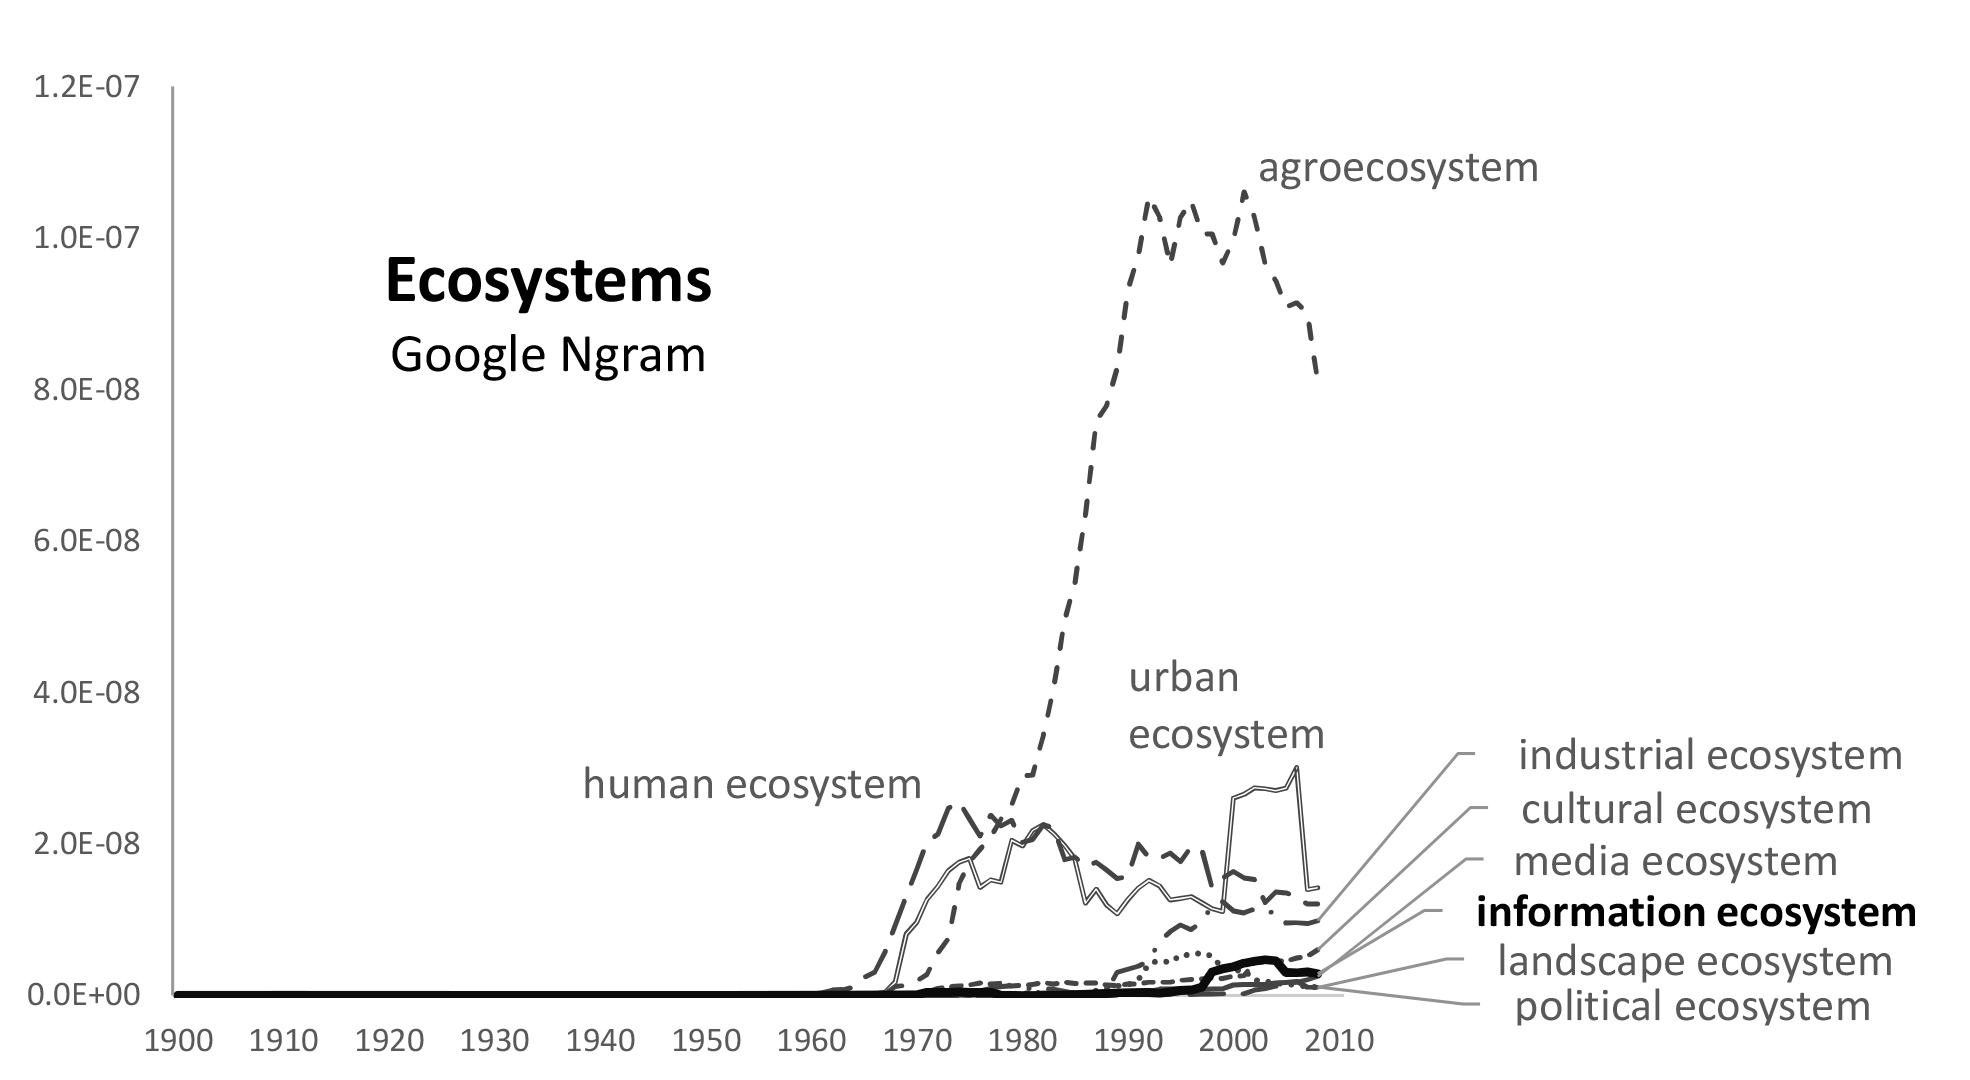
\includegraphics[width=5.5in]{figures/ecosystemsAll}
  \caption{Emergent use varying ecosystem metaphors as a Google Ngram. Compare to figure 2! The use of various ecologies vs various ecosystem metaphors is an order of magnitude higher. It is more common to say information ecology (as a study of information systems using ecological concepts) than it is to say information ecosystem (implying a metaphorical relationship). Note that agro ecology is an exception. While some might say this is a human made ecosystem, it is perhaps more correct to think of it as a human \textit{influenced} ecosystem.}
\end{figure}

Within the academy information ecology is an ecological approach to answering research questions. This might mean using some tools from the ecology toolkit or even thinking broadly about the function of information in mediating relationships between the living and the non-living. On the other hand, an information ecology in the business management literature is the connectedness, the inter-relatedness, the actual set of relationships between human actors, machines and the information itself. It could even refer to the social environment or human community in which information is flowing. In the business management literature an information ecology is almost synonymous with an information ecosystem, yet it rarely has a connection to the natural environment.